

\section*{Combining plots}
It is possible to combine two plots. We used the graphical parameters command \texttt{par()} to create an array. 
Often we just require two plots side by side or above and below. We simply specify the numbers of rows and columns of this array using the \texttt{mfrow} argument, passed as a vector.

<code>
par(mfrow=c(1,2))
plot(x,y1)			# draw first plot
plot(x,y2)			# draw second plot
par(mfrow=c(1,1))		# reset to default setting.
</code>

#### *{Combining Plots}
Multiple plots can be combined into a single graph, arranged vertically, horizontally or in a grid.

This can be implemented with \texttt{\textbf{par( )}} function, specifying the arrangment using the \texttt{\textbf{mfrow=}} argeument.

Suppose we require a histogram above a boxplot (with horizontal orientation). If we consider this as a grid, we have an array of two rows, with one column.

<pre>
<code>
# 2 plots arranged in 2 rows and 1 column


par(mfrow=c(2,1))


hist(mtcars$wt, main="Histogram of wt",col=c("lightblue","blue"))
boxplot(mtcars$
wt, main="Boxplot of wt",horizontal=TRUE,col="lightblue")

</code>
</pre>

%\begin{center}[h1]
%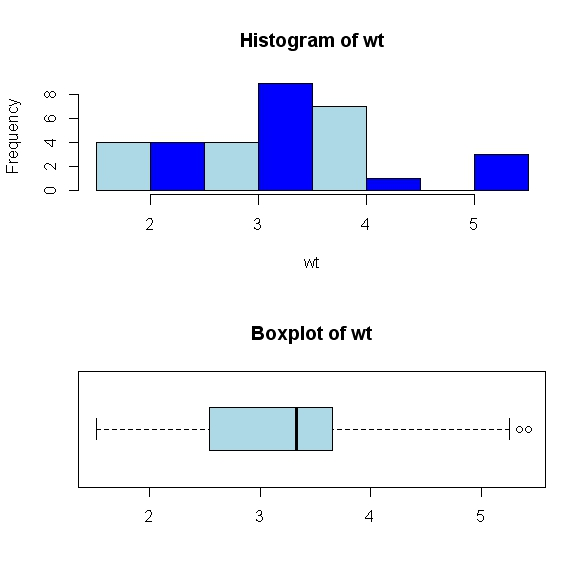
\includegraphics[scale=0.65]{combiPlot}
%\end{center}



\end{document}
